% Document template suitable for use as a LaTeX master-file 
% for thesis works in University of Turku Department of Computing
%
% Technical usage guide: https://tech.utugit.fi/soft/thesis/doc/doc/overview/
% 

\documentclass[language=finnish,version=final,mainfont=none,sharelatex=false]{utuftthesis}
\setcounter{secnumdepth}{2}
\setcounter{tocdepth}{2}
\usepackage{float}
\usepackage[caption=false]{subfig}
\usepackage{biblatex}

\usepackage{listings}
\lstset{basicstyle=\small,breaklines=true}

% Define the algorithm environment
%\makeatletter
\providecommand\textquotedblplain{%
  \bgroup\addfontfeatures{Mapping=}\char34\egroup}
\providecommand{\tabularnewline}{\\}
\floatstyle{ruled}
\newfloat{algorithm}{tbp}{loa}
\providecommand{\algorithmname}{Algoritmi}
\floatname{algorithm}{\protect\algorithmname}
%\makeatother

\addbibresource{bibliografia.bib}

\begin{document}

\pubyear{2023}
\pubmonth{12}
\pubtype{tkk}
\title{Muistinhallinnan tekniikat sulautetuissa järjestelmissä}
\author{Matias Suksi}

\maketitle
\keywords{sulautettu järjestelmä, muistin allokointi, staattinen allokointi, dynaaminen allokointi, keko, pino, reaaliaikaisuus}

\begin{abstract}

Sovelluksen tehokas muistinkäyttö on tärkeää sujuvan käyttökokemuksen takaamiseksi, ja sulautetuissa järjestelmissä tämä sujuvuus korostuu entisestään. Tutkielmassa tutkitaan minkälaisia muistinhallinnan tekniikoita voidaan hyödyntää sulautetuissa järjestelmissä. Tutkielmassa käydään läpi sovelluksen muistin rakennetta, esitellään mitä rajoitteita ja haasteita sulautetut järjestelmät aiheuttavat tehokkaalle muistinhallinnalle.

Tutkielmassa havaitaan, että staattiset muistinhallinnan menetelmät ovat monesti suorituskyvyn kannalta tehokkaampia kuin dynaamiset menetelmät. Kuitenkin monesti sulautettujen järjestelmien vaatimukset aiheuttavat sen, kuten reaaliaikaisuus, että joudutaan tyytyymään dynaamiseen muistinhallintaan. Tutkielma ei kykene tuottamaan yleistystä, mitkä muistinhallintatekniikka ovat tehokkaimpia sulautetuissa järjestelmissä, vaan tutkielmassa havaitaan, että muistihallintatekniikan sovellus on täysin riippuvainen sovelluskohteesta. Täten myös tutkielmassa esitellyt muistinhallinan tekniikat ovat valittu tutkielmaan lähdekartoituksessa useimmiten vastaan tulleina muistirakenteita, joita sulautettuun järjestelmään on pyritty soveltamaan. Tutkielmassa havaittuja sulautettujen järjestelmien haasteita ovat mm. laitteiston rajoitteet, järjestelmän vaatimukset ja käyttökohde. Muitakin muistinhallintatekniikoita ja -rakenteita on olemassa paljon, ja näitä onkin syytä tutkia mahdollisissa jatkotutkimuksissa.

\end{abstract}



% mandatory
\tableofcontents

% change the name if the default doesn't sound right
\renewcommand{\algorithmname}{\listingscaption}

% The thesis starts here.

\begin{comment}
To better organize things, create a new tex file for each chapter
and input it below.

Avoid using the å, ä, ö or <space> characters in referred names and
underscores \_ in file names (may break hyperref).

Good luck!
\end{comment}

\chapter{Johdanto} \label{Johdanto}


\chapter{Muistinhallinta} \label{Toinen luku}

Ohjelman muistin rakenteen ymmärtäminen on erityisen tärkeää tehokkaan muistin käytön saavuttamiseksi. Seuraavassa luvussa tullaan esittelemään miten muistin allokointi ohjelmissa toimii
ja millaisista muistialueista ohjelman muisti koostuu. Huomioitavaa on, että seuraavaksi esiteltävä sovelluksen muistin rakenne, on tyypillisin malli kuvaamaan, miten tietokoneohjelman muisti koostuu. Ohjelman muistin rakenteeseen vaikuttaa mm. käytössä oleva suoritinarkkitehtuuri, ohjelmointikielen kääntäjä sekä kääntäjien tarjoamat muistin optimointityökalut.

\section{Ohjelman muisti}

Ohjelman suorituksen aikainen muisti jakautuu erilaisiin muistialueisin. Koodiosa sisältää varsinaisesti ajettavan ohjelman binäärin eli ohjelmatiedoston, jonka prosessori suorittaa. Lisäksi ohjelmalla on olemassa dataosa, joka koostuu alustetusta datasta ja alustamattomasta datasta. Alustetun datan alueeseen kuuluvat globaalit ja staattiset muuttujat sekä vakioarvoiset muuttujat, joille on alustettu jokin arvo. Alustamattomassa data-alueessa on kaikki alustamaton data eli muuttujat, jotka ovat esitelty (declare), mutta joille ei ole annettu mitään arvoa. Näiden muistialueiden data allokoidaan ajettavan ohjelman muistiin jo käännön aikana (engl. \textit{compile time}) eli ohjelmointikielen kääntäjän kääntäessä lähdekoodin. Ohjelmalla on lisäksi myös kaksi muuta muistialuetta, pino ja keko. Tyypillisesti pino sijaitsee ylhäällä ja keko alhaalla ohjelman virtuaalisessa muistiavaruudessa.\cite{mmic2010} Pinon datan allokointi tapahtuu jo käännön aikana, kun taas keon datan allokointi tapahtuu vasta ohjelman ajon aikana (engl. \textit{runtime})\cite{ddm2015book}. Pinon allokoinnin määrittely ei ole aivan yksikäsitteistä. Yleisesti lähteissä määritellään, että allokointi tapahtuu käännön aikana, mutta jotkin lähteet määrittelevät, että allokointi tapahtuu ajon aikana. Tämä johtuu pinon allokoinnin luonteesta, sillä vaikka pinon hallintaan liittyvät ohjeet syntyvät jo käännön aikana, varsinainen itse datan osoitteistus tapahtuu ajon aikana.

\begin{figure}[tbh]
{\begin{centering}
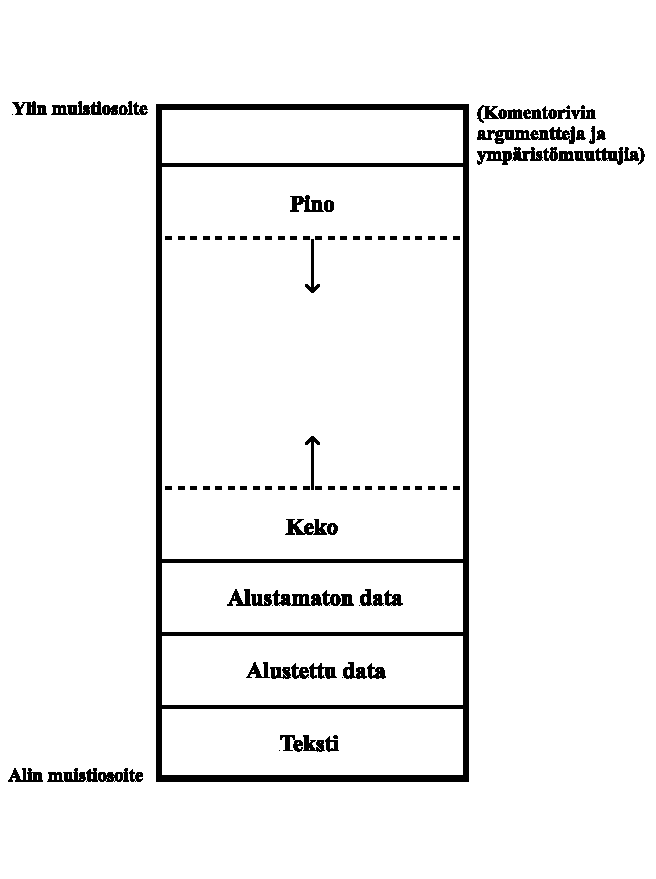
\includegraphics[width=0.6\textwidth]{kuvat/muistin_rakenne.pdf}
\par\end{centering}}
\caption{Ohjelman muistin rakenne \cite{mmic2010} (suomennettu kuva lähteestä)}
\end{figure}

\subsection{Pino}

Pino (engl. \textit{stack}) on ohjelman muistialue, johon allokoidaan paikalliset muuttujat, funktioiden parametrit ja paluuosoitteet. Se noudattaa LIFO-periaateetta (engl. \textit{Last In First Out}) eli pinoon viimeiseksi puskettu data poistetaan pinosta myös ensimmäisenä. LIFO-periaatteen ansiosta pinoallokointi on tyypillisesti nopeampaa kuin kekoon allokoiminen, johtuen tavasta, miten pinon dataan päästään käsiksi. Lisäksi, pinon tavuja käytetään ohjelmassa säännöllisesti yhä uudelleen ja uudelleen, jolloin ne säilyvät hyvin prosessorin nopeassa välimuistissa. Data allokoidaan pinoon automaattisesti ja poistetaan sieltä, kun sen näkyvyysalue päätyy. Pino koostuu kehyksistä (engl. \textit{frame}), joita pusketaan pinoon, kun ohjelma aloittaa uuden funktiokutsun suorittamisen. Tyypillisesti pinon koko on päätetty ennen ohjelman suorituksen aloittamista, ja pinoon allokoitavien muuttujien koko on tiedettävä etukäteen jo ennen kääntöä.\cite{mmic2010}
Pino-osoitin (engl. \textit{stack pointer}) pitää yllä tietoa muistiosoitteesta, jossa pinon viimeinen elementti sijaitsee. Tätä osoitinta muuttamalla, ohjelma pitää yllä tietoa mihin uusi kehys lisätään tai mistä vanha kehys poistetaan. Pino-osoittimen arvo pienenee, kun dataa pusketaan pinoon ja vastaisuudessa kasvaa, kun dataa poistetaan pinosta (huomioi pinon sijainti ohjelman muistiavaruudessa, kts. kuva 2.1).\cite{sasp2006}

\subsection{Keko}

Keko (engl. \textit{heap}, suom. myös \textit{kasa}) on muistialue, johon kehittäjä allokoi sekä josta myös vapauttaa muuttujat manuaalisesti. Keko sisältää käytettävissä olevien ja vapaiden muistilohkojen linkitetyn listan. Keolle annetaan aloituskoko ohjelman suorituksen alkaessa, mutta muistinvaraaja voi pyytää sitä lisää tarvittaessa käyttöjärjestelmältä. Vastapainona pinolle, keko on hyödyllinen, kun ei voida tietää etukäteen kuinka paljon muistia tarvitsee varata ajon aikana.\cite{mmic2010} On syytä mainita, että tietokoneohjelman muistialue keko ei ole sama asia kuin tietorakenne keko.

\section{Muistin allokointi ohjelmointikielissä}

Tietokone ohjelman käyttämä muisti voidaan jakaa kahden tyyppisen muistiin, staattiseen ja dynaamiseen muistiin. Staattisella muistilla tarkoitetaan yleensä globaalia data-aluetta ja pinoa, kun taas dynaamisella muistilla viitataan yleensä kekoon.\cite{ddm2015book}

***Staattinen muistinhallinta***

Dynaamista muistinhallintaa varten ohjelmointikielet tarjoavat erilaisia valmiista kirjastoista saatavia funktioita muistin varausta ja vapautamista varten. C-ohjelmointikielessä funktio, jolla varataan muistia on malloc(), joka ottaa vastaan argumenttina muistin koon tavuina. Muistia vapautetaan funktiolla free(), joka ottaa parametrina osoittimen osoittaman muistilohkon. Lisäksi, on olemassa calloc() ja realloc(), joilla voi myös varata muistia. Calloc() ottaa kaksi argumenttia, joista toinen on varatun muistilohkon koko ja toinen määrittää kuinka monta näitä lohkoja varataan. Malloc()- ja calloc()-funktioiden keskeinen ero on, että calloc()-funktio myös alustaa varatun muistialueen nolliksi. Malloc() ei tätä alustusta suorita, vaan malloc()-funktion varaama muistialue sisältää mielivaltaisia alustamattomia arvoja. Realloc() on funktio, jolla pystyy muokkaamaan jo aikaisemmin varatun muistialueen kokoa. Realloc() ottaa argumentikseen muokattavan muistialueen osoittimen sekä muistilohkon uudelleen määritetyn koon.\cite{c2015book}

Muistivuoto on muistinkäytön ongelmatilanne, joka tapahtuu kun ohjelma käyttää muistia, mutta ei kykene vapauttamaan sitä takaisin käyttöjärjestelmän käyttöön. Muistivuodot ovat hyvin ikäviä ongelmatilanteita, sillä niiden jäljittäminen vaatii pääsyn ohjelman lähdekoodiin, ja monesti muistivuodot ilmenevät ohjelmassa lukuisina muina ongelmina. Usein ajatellaan virheellisesti, että yleisesti ohjelman lisääntynyt muistinkäyttö on muistivuoto, vaikka tämä ei pidä paikkaansa. Monesti muistivuodot eivät ilmene ohjelmaa ajettaessa välittömästi, vaan hitaasti ohjelman ajon aikana, kun ohjelma varaa yhä enemmän ja enemmän muistia. Lopulta tämä ilmenee ohjelman kaatumisena tai käyttöjärjestelmän hidastumisena.\cite{mmic2010}

Dynaaminen muistinhallinta tuo kehittäjälle vapautta, mutta myös suuren vastuun. Aikaisemmin mainitut muistinkäytön ongelmatilanteet ja virheet voivat aiheuttaa päänvaivaa kokemattomalle kehittäjälle, mutta kokeneelle kehittäjälle osoittimet ja manuaalinen allokointi tarjoavat tehokkaat työkalut sovelluksen muistinkäytön tehostamiselle. Ohjelmointikielissä, jotka tarjovat kehittäjälle dynaamisen muistinhallinnan mahdollisuuden, kehittäjän on hyvin tärkeää ymmärtää, miten ohjelman muisti toimii, jotta näiltä onglematilanteilta vältytään.

Ohjelmalistaus 1 on käytännön esimerkki, joka havainnollistaa mihin muistialueeseen kukin koodirivi sijoittuu ohjelman muistissa.

\begin{algorithm}[tbh]
\begin{lstlisting}[language=C]
#include <stdio.h>
#include <stdlib.h>

//Alustamaton muuttuja --> alustamaton data
int i;
//Alustettu muuttuja --> alustettu data 
int n = 1; 

//Funktiokutsu --> Pino
int main(void)  
{  
    //Paikallinen muuttuja --> Pino
    int numero = 10;
    //Dynaamisesti allokoitu muistilohko --> Keko    
    int* osoitin = (int*)malloc(n * sizeof(int));
    //Dynaamisesti vapautettu muistilohko --> Vapautettu keosta  
    free(osoitin);
    return 0;
}
\end{lstlisting}
\caption{Demonstraatio muistin allokoinnista C-ohjelmointikielessä\label{alg:Demonstraatio}}
\end{algorithm}
\chapter{Kolmannen luvun otsikko} \label{Kolmas luku}

Tässä luvussa tarkastellaan kahden kuvan upottamista samaan kelluvaan
kuvaympäristöön (Kuva \ref{fig:Optimointia-kahdella-eri}).

\begin{figure}[tbh]
\subfloat[Käynnistysajan optimointi Nailgunilla.]{\begin{centering}
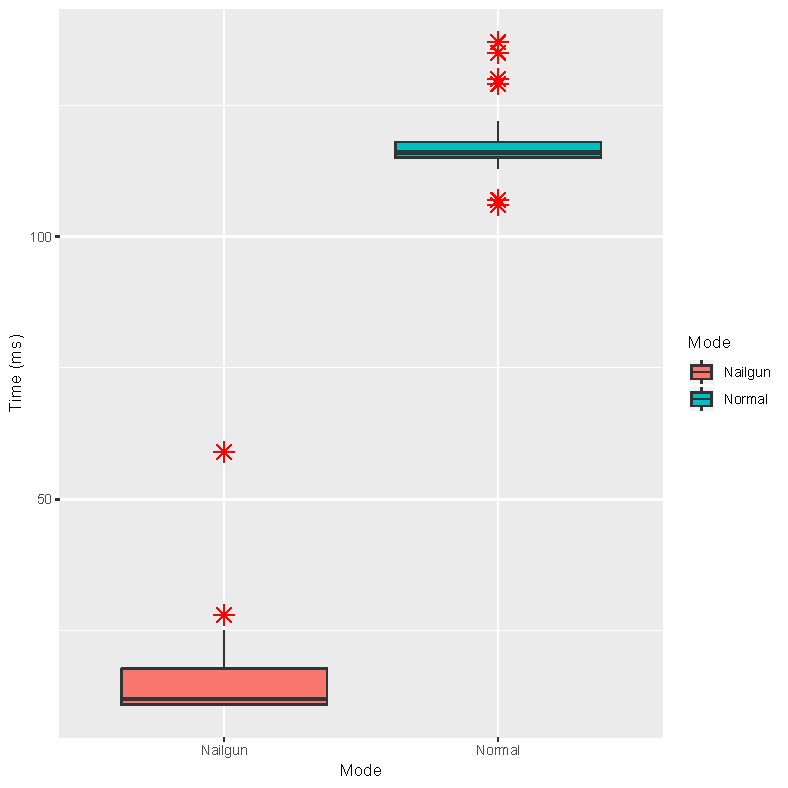
\includegraphics[width=0.45\textwidth]{kuvat/nailgun.pdf}
\par\end{centering}
}\subfloat[Koon optimointi Proguardilla.]{\begin{centering}
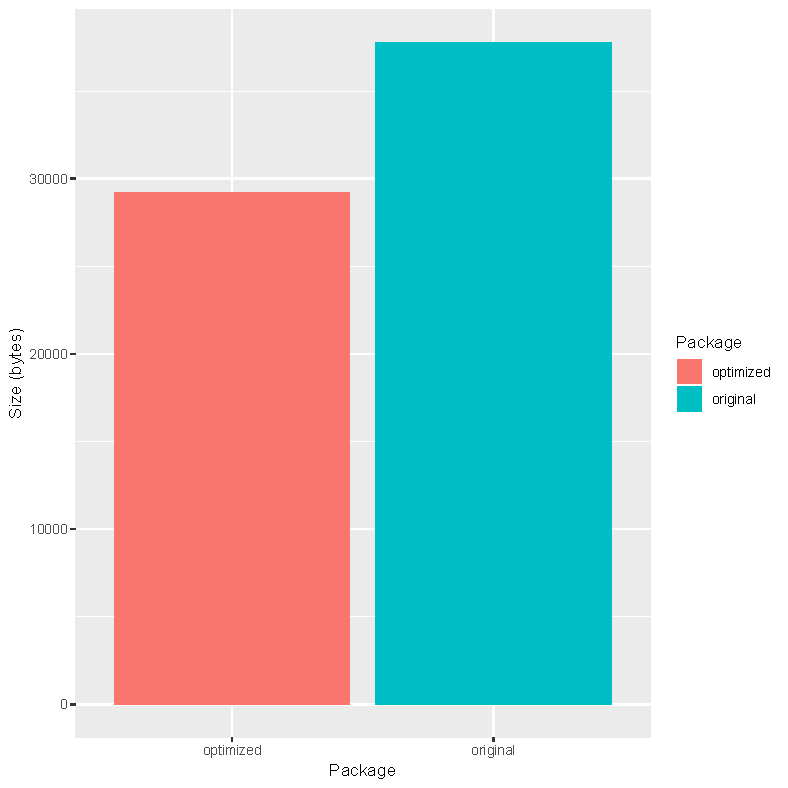
\includegraphics[width=0.45\textwidth]{kuvat/proguard.pdf}
\par\end{centering}
}\caption{Optimointia kahdella eri tavalla.\label{fig:Optimointia-kahdella-eri}}

\end{figure}
\chapter{Muistinhallinan tekniikoita ja rakenteita} \label{Neljäs luku}

Tässä luvussa tullaan esittelemään yleisiä muistinhallinan tekniikoita, joita voidaan hyödyntää sulautetuissa järjestelmissä.

\section{Rengaspuskuri}

Rengaspuskuri (engl. \textit{circular buffer} on järjestetty tietorakenne, jossa viimeisen alkion jälkeen palataan takaisin ensimmäiseen alkioon. Yleensä rengaspuskuri toteutetaan, joko järjestettynä taulukkona tai linkitettynä listana, jonka viimeinen alkio osoittaa takaisin ensimmäiseen alkioon. Rengaspuskurin etuindeksi (engl. \text{front index}) osoittaa tyhjän paikan, johon seuraavaksi lisättävä alkio laitetaan. Takaindeksi (engl. \text{back index}) osoittaa seuraavaksi poistettavan alkion paikan. Rengaspuskurit ovat erittäin yleisiä tietorakenteita juuri reealiaikaisissa sulautetuissa järjestelmissä, joissa useat prosessit kommunikoivat keskenään. Rengaspuskuri toimii väliaikaisena muistina prosesseille, jolloin prosessit voivat toimia asynkronisesti.\cite{c2015book}

Seuraavaksi esitellään yksinkertaisen kokonaislukuja sisältävän rengaspuskurin totetus.

\begin{algorithm}[tbh]
\begin{lstlisting}[language=C]
typedef struct RengasPuskuri_t {
    int* taulukko;  //Osoitin taulukkoon
    int koko;       //Maksimikoko
    int alkioiden_lukumaara;    //
    int ensimmainen_alkio;  //Indeksi puskurin alkuun
    int viimeinen_alkio;    //Indeksi puskurin loppuun
}
\end{lstlisting}
\caption{Rengaspuskurin implementaatio\label{alg:Rengaspuskuri}}
\end{algorithm}

\section{Segmentoitu pino}

Suurin osa ohjelmista käyttävät aikaisemmassa luvussa esiteltyä pinoa yhtenä muistirakenteena. Tällaista pinoa voidaan tarkemmin nimittää jatkuvaksi pinoksi (engl. \textit{contiguous stack}), sillä tämäntapainen pino varaa yhtenäisen muistialueen ohjelman muistiavaruudesta. Tällaisella perinteisellä jatkuvalla pinolla on kuitenkin heikkouksia sulautetuissa järjestelmissä. Muisti allokoidaan pinolle staattisesti eli jo ennen ohjelmakoodin kääntöä, jolloin pinon maksimikoko ajonaikana on ennaltamääritety. Lisäksi jatkuvan pinon ylivuoto (engl. \textit{stackoverflow}) on vaikea havaita, sillä monesti sulautetuissa järjestelmissä käytettävissä matalan tason mikrokontrollereista puuttuu kokonaan muistinsuojausyksikkö (engl. \textit{MPU, memory protection unit}), jolla ylivuoto voitaisiin havaita. Lisäksi muut vaihtoehtoiset menetelmät ylivuodon tunnistamiseen ovat monesti muistinkäytön tehokkuuden kannalta hyvin tehottomia, ja joita monet yleiset sulautetut ohjelmointikielien kääntäjät eivät tue tai tukevat hyvin heikosti. Näistä kääntäjistä esimerkkejä ovat ARM GNU ja LLVM.\cite{bsstes@2023}

Jatkuvan pinon vastapainona on segmentoitu pino (engl. \textit{segmented stack}), joka eroaa jatkuvasta pinosta niin, että pino on jaettu pienempiin erillisiin pienempiin pinoihin (engl. \textit{stacklet}), jolloin säikeet ja funktiot sekä niiden data allokoidaan omissa pinoissaan. Nämä pienemmät pinot allokoidaan dynaamisesti keosta. Segmentoitu pino on harvoin käytetty muistirakenne, koska sillä on tunnetusti huono suorituskyky ja muistinkäyttö on tehotonta. Kuitenkin, monissa mikrokontrolleripohjaisissa järjestelmissä, joita sulautetuissa järjestelmissä paljon käytetään, nämä suorituskykyongelmat häviävät. Lisäksi pinon ylivuototilanteet on helppo selvittää, sillä pääpinon sisällä olevaa pinoa voidaan dynaamisella allokoinnilla kasvattaa tarpeen vaatiessa. Ajon aikainen kirjasto, joka allokoi ja vapauttaa segmentoidun pinon pienempiä pinoja, kohtelee tätä muistirakennetta linkitettynä listana.\cite{bsstes@2023}

Segmentoitu pinon hyöty sulatetuissa järjestelmissä on aikaisemmin mainittujen haittojen häviäminen ja uusien muistin optimointimahdollisuuksien syntyminen.

Heikkoudet häviävät:
    1. Muistin fragmentoituminen vähenee
    2. Koodikannan kontrollin paraneminen
    3. Suorituskyvyn heikentyminen on hyväksyttävämpää

Uusia mahdollisuuksia syntyy:
    1. Muistinkäytön turvallisuus voidaan saavuttaa ohjelmointikielen kääntäjällä
    2. Laitteisto- ja energiatehokkuus

\section{Buddy Memory Allocation}
\section{Memory Pooling}
\section{Fixed-size Block Allocation}
\section{Memory Banks}
\section{Object Pools}
\section{Slab allocation}
\chapter{Muistinhallintatekniikoiden analysointi ja suorituskyvyn mittaaminen sulautetuissa järjestelmissä} \label{Kuudes luku}

Tässä luvussa pyritään summaamaan edellisen luvun menetelmiä sekä esitellään miten sulautetun järjestelmän muistinkäyttöä voidaan mitata ja arvioida.

\section{Tekniikoiden analysointi}

Monet viitatut ja lähdekartoituksessa tutkitut artikkelit lähtevät lähtökohdasta, että halutaan toteuttaa staattinen menetelmä, sillä ne ovat tunnetusti nopeampia muistinkäytön kannalta kuin dynaamiset menetelmät. Staattisen allokoinnin suurin etu on se, että sillä kyetään vastaamaan reaaliaikaisuuden asettamiin haasteisiin parhaiten ja staattiset menetelmät ovat stabiilimpia kuin dynaamiset\cite{daroemmfera@2006}. Kuitenkin monesti joudutaan tyytymään dynaamiseen ratkaisuun, sillä staattisen allokoinnin luonne aiheuttaa liian paljon rajoituksia tehokkaan ratkaisun tuottamiseen. Täten käsitellyt artikkelit ja niin myös tämä tutkielma, keskittyy pääasiassa dynaamisiin menetelmiin sekä niiden kehittämiseen ja optimointiin. Tutkielmaa varten lähteistöä staattisista muistinhallintatekniikoista sekä hybridimalleista, jotka koostuivat dynaamisista ja staattisista piirteistä löytyi, mutta ne sivuutettiin tutkielmasta niiden vaativuuden sekä kompleksisuuden takia.

Staattiset allokointimenetelmät ennaltaehkäisevät muistin fragmentoitumista\cite{daroemmfera@2006}. Tämä fragmentoitumisen vähentäminen oli artikkeleissa yhtenä vallitsevana teemana, ja tämä tuntuu olevan keskeisenä ongelmana tehokkaan muistinhallinnan kehittämisessä sulautetuissa järjestelmissä. Monissa artikkeleissa, jotka käsittelivät dynaamisia menetelmiä, fragmentoituminen listattiin merkittävänä ongelmana ja käsiteltävää dynaamista menetelmää esiteltiin siinä valossa, että miten menetelmä kykenee vastaamaan fragmentoitumisen ongelmiin. Lisäksi tutkielmassa löydettiin uusia keinoja mm. miten ohjelmointikielenkääntäjän avulla voidaan tehostaa sovelluksen muistinkäyttöä.

\section{Suorituskyvyn mittaaminen}

Seuraavaksi esitellyt muistinkäytön tehokkuuden mittarit ovat työkaluja erityisesti reaaliaikaisten sulautettujen järjestelminen dynaamisen muistinkäytön mittaamiseen, mutta nämä ovat muutenkin varsin käyttökelpoisia yleisellä tasolla sulautetuissa järjestelmissä (kts. luku 3.1.1).

\begin{itemize}
\item{A. Suurimman-Pienimmän lohkon mittari (engl. \textit{Smallest-Biggest Block Metric (SBBM)}): Kun sovellus saa pyynnön allokoida muistia, suurin huoli on löytää pyynnöllä tarpeeksi suuri yhtäjaksoinen muistilohko. Fragmentoitumisen takia on mahdollista, että tarpeeksi suurta vapaata muistilohkoa ei ole saatavilla, vaikka järjestelmän yhteenlaskettu vapaa muisti olisikin huomattavasti suurempi kuin pyydetyn muistilohkon koko. SBBM-mittari mittaa ohjelman ajon aikana suurimpien vapaiden lohkojen kokoja, ja lopuksi mittauksen jälkeen, se valitsee näistä lohkoista pienimmän lohkon.

\item{B. Vapaan lohkon mittari - Keskimääräisen koon mittari (engl. \textit{Free Block Metric - Average Size (FBM-AS)}): FBM-AS -mittari ilmaisee ajonaikana vapaiden lohkojen koon keskiarvon.}

\item{C. Sisäinen fragmentoituminen (engl. \textit{Internal Fragmentation (IF)}): IF-mittari mittaa muistin tuhlausta kun muistipyyntöön vastataan suuremmalla lohkolla kuin on välttämätöntä. Muistin tuhlaus on sisäistä suhteessa allokoituun lohkoon. Nythän muistia ei ole pirstoutunut koko ohjelman muistiavaruudessa olevien lohkojen väliin, vaan se on tuhlaantunut itse muistilohkon sisään. Siksi tätä sanotaan sisäiseksi fragmentoitumiseksi.}

\item{D. Kustannuksen mittari (engl. \textit{Cost Metric (CM)}): CM-mittari mittaa järjestelmän tehokkuutta suhteessa saatavilla olevien resurssien määrään. CM-mittari mittaa kuinka paljon muistia järjestelmä vaatii sovelluksen tärkeimpien toiminnallisuuksien suorittamiseen.}

\item{E. Suorituskyvyn mittari (engl. \textit{Performances Metric (PM)}): PM-mittari mittaa muistinhallintajärjestelmän suorituskykyä. Tämä mitataan laskemalla kuinka monta skannausta järjestelmä tarvitsee muistilohkoihin käsiksi pääsyyn. Eli tarkemmin tämä mittari mittaa kuinka nopeasti sovellus löytää pyyntöä vastaavan tarpeeksi ison muistilohkon järjestelmästä, kuinka nopeasti lohko voidaan vapauttaa ja asettaa takaisin oikealle paikalleen vapaiden lohkojen listaan.}

\cite{tmtt@2006}

\end{itemize}


\chapter{Yhteenveto} \label{Yhteenveto}

Tutkielmassa esitellään sovelluksen muistin teoriaa, joka on johdattelua itse sovelluksen muistinhallintaan. Tutkielmassa myös esitellään ja määritellän sulautetun järjestelmän käsite, ja tuodaan esille mitä haastetia sulautetut järjestelmät aiheuttavat kehittäjälle. Tutkielma päättyy erilaisten muistinhallintatekniikoiden esittelyyn, niiden analysointiin ja suorituskyvyn mittaamiseen esittelyyn. Tutkielman edetessä huomataan, että staattinen muistinhallinta aiheuttaa tietynlaisia rajoitteita, jonka takia monesti jäädään keskittymään dynaamisien menetelmien optimointiin.

Tutkielma ei kykene antamaan yhtä oikeaa vastausta päätutkimuskysysmykseen: "millaisia muistinhallinnan tekniikoita voidaan hyödyntää sulautetuissa järjestelmissä". Sulautettuja järjestelmiä on paljon erilaisia ja oikeanlainen tehokas muistinkäytön ratkaisu on täysin tapauskohtainen. Ratkaisua suunnitellessa on otettava huomioon järjestelmän laitteisto, vaatimukset ja käyttökohde. Vaikka tutkielma ei kykene antamaan yksikäsitteistä vastausta ongelmaan, tutkielma esittelee faktoja mitä pitää ottaa huomioon muistinhallintatekniikoiden soveltamisessa sulautetuissa järjestelmissä ja tuo esiin mahdollisia eteentulevia haasteita. Toiseen tutkimuskysymykseen saavutetaan tutkielmassa huomattavasti parempi vastaus, ja tutkielmassa havaitaan, että se onkin vahvasti sidoksissa päätutkimuskysymykseen. Tutkielmassa havaitut päähaasteet ovat juuri edm. mainitut laitteiston rajoitteet, järjestelmän vaatimukset ja käyttökohde. Tutkielmassa mainittuja laitteiston rajoitteita ovat mm. tuotantokustannukset, virrankulutus ja laitteiston fyysinen koko. On tärkeää muistaa, että rajoitteita on muitakin ja monet rajoitteet syntyvät johdannaisina näistä kolmesta keskeisestä rajoitteesta tai niiden yhdistelmästä. Tästä esimerkkinä mainittakoon, että mm. tietokoneen fyysinen koko ja tuotantokustannukset aiheuttavat näistä johtuvan rajoitteen kuin järjestelmän rajallinen muistin määrä.

Tukielman aiheeseen liittyvää käsitteistöä on hyvin paljon, minkä takia tämä tutkielma on hyvin teoriapainoitteinen pintapuolinen katsaus aiheeseen. Tutkielmaa voisi laajentaa tulevaisuudessa mm. kokeellisella tutkimuksella, jossa testattaisiin eri muistinhallintatekniikoiden suorituskykyä erityppisissä sulautetuissa järjestelmissä ja toteuttamalla yksityiskohtaisempaa analyysiä muistinhallintatekniikoista. Kattavammalla tutkielmalla voitaisiin saavuttaa jonkinlainen yleistys, että minkälaiset tekniikat ovat tehokkaita tietyntyyppisissä sulautetussa järjestelmässä.

% The thesis main content ends here.

\printbibliography

\begin{comment}
Important! Create the appendix chapters with command \textbackslash appchapter\{some
name\} instead of \textbackslash chapter\{some name\} for the automagic
page counting to work!
\end{comment}

\end{document}
